\documentclass[11pt, addpoints, answers]{exam}

\usepackage{amsmath, amssymb}
\usepackage{xcolor}
\usepackage{enumerate}
\usepackage{graphicx}
\usepackage{tabularx}
\usepackage{algorithm}
\usepackage{algpseudocode}
\usepackage{tikz}
\usepackage{tikz-qtree}
\usepackage{subfigure}

\newcommand{\red}[1]{\textcolor{red}{#1}}
\newcommand{\blue}[1]{\textcolor{blue}{#1}}

% For inserting code snippets.
\usepackage{listings}
\lstset{
    columns = fixed,
    basewidth = {0.5em},
    breaklines = true,
    backgroundcolor = \color{white},
    keywordstyle = \color[RGB]{40, 40, 255},
    numberstyle = \footnotesize\color{darkgray},
    commentstyle = \ttfamily\color{violet},
    basicstyle = \ttfamily,
    stringstyle = \ttfamily\color[RGB]{128, 0, 0},
    showstringspaces = false,
    language = {[11]C++},
    escapechar = \@
}
\lstnewenvironment{cpp}[1][]{\lstset{language = {[11]C++}, #1}}{}

\renewcommand{\baselinestretch}{1.15}
\setlength{\parskip}{1.25\baselineskip}

\usepackage{tikz}
\usepackage{tikz-qtree}
\tikzset{every tree node/.style={minimum width=2em,draw,circle},
    blank/.style={draw=none},
    edge from parent/.style=
    {draw,edge from parent path={(\tikzparentnode) -- (\tikzchildnode)}},
    level distance=1.2cm}



% headers, footers, titles
\newcommand{\CourseName}{CS101 Algorithms and Data Structures}
\newcommand{\HomeworkNO}{6}
\newcommand{\DueDate}{November 11, 2024}

\pagestyle{headandfoot}
\runningheadrule
\runningheader{CS101 Fall24}{Homework \HomeworkNO}{Due on: \DueDate}
\runningfooter{}{\thepage}{}

\title{
    \vspace{25pt}
    \LARGE ShanghaiTech University \\
    \bigskip
    \textbf{\CourseName} \\
    \textbf{Fall 2024}   \\
    \bigskip
    Homework \HomeworkNO
}
\author{}
\date{Due date: \DueDate, at 23:59}

% formats of questions, choices, points, etc.
\qformat{\bf\thequestion. (\totalpoints\ points) \thequestiontitle\hfill}
\pointname{'}
\CorrectChoiceEmphasis{\bf\color{blue}}
\SolutionEmphasis{\color{blue}}

% We frequently use this font.
\newcommand{\ttt}{\texttt}
\newcommand{\bluett}[1]{\textcolor{blue}{\ttt{#1}}}

\begin{document}

\maketitle

\vspace{50pt}

\begin{enumerate}
    \item Please write your solutions in English.
    \item Submit your solutions to Gradescope.
    \item Set your FULL name to your Chinese name and your STUDENT ID correctly in Gradescope account settings.
    \item If you want to submit a handwritten version, scan it clearly. \ttt{CamScanner} is recommended.
    \item We recommend you to write in \LaTeX.
    \item When submitting, match your solutions to the problems correctly.
    \item No late submission will be accepted.
    \item Violations to any of the above may result in zero points.
\end{enumerate}
\newpage

\begin{questions}

\titledquestion{Multiple Choices}

Each question has \textbf{one or more} correct answer(s). Select all the correct answer(s). For each question, you will get 0 points if you select one or more wrong answers, but you will get 1 point if you select a non-empty subset of the correct answers.

Write your answers in the following table.

%%%%%%%%%%%%%%%%%%%%%%%%%%%%%%%%%%%%%%%%%%%%%%%%%%%%%%%%%%%%%%%%%%%%%%%%%%%
% Note: The `LaTeX' way to answer a multiple-choice question is to replace `\choice'
% with `\CorrectChoice', as what you did in the first question. However, there are still
% many students who would like to handwrite their homework. To make TA's work easier,
% you have to fill in your selected choices in the table below, no matter whether you use 
% LaTeX or not.
%%%%%%%%%%%%%%%%%%%%%%%%%%%%%%%%%%%%%%%%%%%%%%%%%%%%%%%%%%%%%%%%%%%%%%%%%%%

\begin{table}[htbp]
	\centering
	\begin{tabular}{|p{2cm}|p{2cm}|p{2cm}|p{2cm}|p{2cm}|}
		\hline 
		(a) & (b) & (c) & (d)  \\
		\hline
  		%%%%%%%%%%%%%%%%%%%%%%%%%%%%%%%%%%%%%%%%%%%%%%%%%%%%%%%%%%
		% YOUR ANSWER HERE.
		   &  &  &  \\
            %%%%%%%%%%%%%%%%%%%%%%%%%%%%%%%%%%%%%%%%%%%%%%%%%%%%%%%%%%
		\hline
	\end{tabular} 
\end{table}

\begin{parts}


\part[2] Which of the following statements about topological sort is/are true?
\begin{choices}
    \choice A sub-graph of a DAG may not have a topological sorting.
    \choice Any directed tree has a topological sorting.
    \choice It's possible for a DAG to have multiple topological sortings.
    \choice Since we have to scan all vertices to find those with zero in-degree in each iteration, the run time of topological sort is $\Omega(|V|^2)$.
    
\end{choices}

\part[2] Which of the following statements about topological sort is/are true?

\begin{choices}

\choice For a connected graph, we can determine if it has a cycle in $\Theta(|E|)$ time.

\choice A critical path in a DAG is a path from the source to the sink with the maximum total weights.

\choice A DAG with all different weighted edges has one unique critical path.


\choice A DAG has at least one source and at least one sink.


\end{choices}

\part[2] Which of the following sequences is/are \textbf{Topological Sorting}(s) of the given DAG?
	\vspace{0.1in}
	\begin{center}
		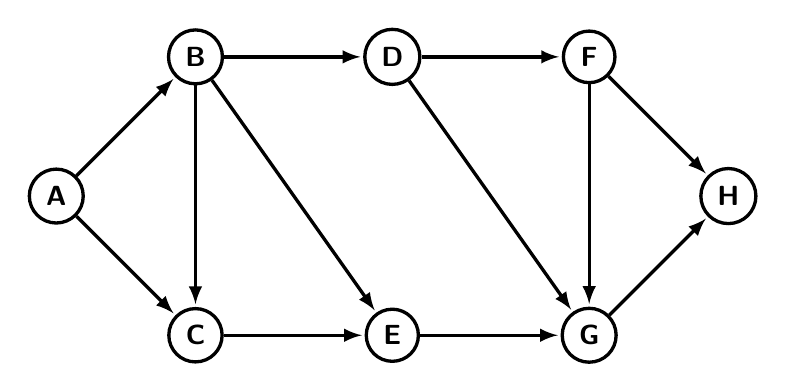
\begin{tikzpicture} [node distance = 2.5cm, very thick, main/.style = {draw, circle, font=\sffamily\bfseries}, edge/.style={->,> = latex, shorten > = 1pt}]
			\node[main] (B) {B};
                \node[main, below left of = B] (A) {A};
			\node[main, below  right of = A] (C) {C};
			\foreach \i\j in {B/D, D/F, C/E, E/G} {
					\node[main, circle, right of = \i] (\j) {\j};
				}
                \node[main, below right of = F] (H) {H};
			\draw[edge] (A) -- (B);
			\foreach \i\j in {B/C, A/C, B/D, D/F, C/E, E/G, B/E, D/G, F/H, G/H} {
					\draw[edge] (\i) -- (\j);
				}
			\draw[edge] (F) -- (G);
		\end{tikzpicture}
	\end{center}
	\begin{choices}
    	\choice 	    A B C E G D F H
		\choice 	A B C D E F G H
		\choice 	A B D C F E G H
		\choice 	    A B D E C F G H
	\end{choices}

\part[2]For the coin-changing problem, denote
    \begin{itemize}
        \item $C=(c_1, c_2,\cdots,c_k)$: the denominations of coins, where $1=c_1<c_2<\dots<c_k$;
        \item $X_n^*$: an optimal solution, i.e., a multi-set of coins which has the minimum number of coins to make change for $n$;
        \item $X_n$: the greedy solution, solved by
        \[
        X_n=\begin{cases}
        \{ \},&n=0\\
        \{c_t\}\cup X_{n-c_t},&n\ge 1, \text{where } c_t=\max\limits_{c_i\le n}c_i \text{ is the largest coin that can be used}
        \end{cases}
        \]
    \end{itemize}

For example, if $C=(1,2,3)$, then $X_4^*$ can be either $\{2,2\}$ or $\{3,1\}$, and $X_4=\{3,1\}$.

Which of the following statements is/are true?

    \begin{choices}
 
        \choice If $\forall i\in[3,n], c_i=c_{i-1}+c_{i-2}$, then $\forall n,|X_n^*|=|X_n|$.
        \choice $\exists C,\exists i$ with $2c_i>c_{i+1}$, such that $\forall n,|X_n^*|=|X_n|$.
        \choice If $\forall i, 2c_i\le c_{i+1}$, then $\forall n,|X_n^*|=|X_n|$.
        \choice If $\forall i\in[2,n], \dfrac{c_i}{c_{i-1}}$ is an integer, then $\forall n,|X_n^*|=|X_n|$.
 
    \end{choices}

\end{parts} 

\newpage



\titledquestion{BST and AVL Tree}

In this question we are going to see what's the difference between general Binary Search tree and AVL tree.

\textbf{Note: We uniformly stipulate that when erasing a non-leaf node $x$, we will fill its successor (the minimum value greater than $x$ among all child nodes) to its original position. If $x$ has no successor, we will fill its predecessor (the maximum value less than $x$ among all child nodes) to its original position.}

\begin{parts}

\part[3] Given an empty Binary Search tree, insert the sequence of integers $15, 20, 23, 10, 7, 5, 30, 25$ from left to right into the tree. Draw the final BST.

\begin{solution}

\vspace{2in}

\end{solution}

\part[3] Given an empty AVL tree, insert the same sequence in part (a), draw the final AVL tree.

\begin{solution}

\vspace{2in}
    
\end{solution}

\part[3] For the final AVL tree in the question above, delete $7$. Draw the AVL tree after deletion.

\begin{solution}

\vspace{2in}

\end{solution}

\part[5] For an AVL tree, define D = the number of descendants of the left child of the root - the number of descendants of the right child of the root. Then what is the maximum of D for an AVL tree with height n? 

$D_{max}=k_1\times 2^n+k_2\times B^n+k_3\times(-\frac{1}{B})^n$, please write down the value of B and $k_i$.
\begin{solution}

\vspace{2in}

\end{solution}
    
\end{parts}

\newpage

\titledquestion{AVL tree operations}

Here is an AVL tree. Denote it as $T$.

\textbf{Note Again: We uniformly stipulate that when erasing a non-leaf node $x$, we will fill its successor (the minimum value greater than $x$ among all child nodes) to its original position. If $x$ has no successor, we will fill its predecessor (the maximum value less than $x$ among all child nodes) to its original position.}

\begin{center}
    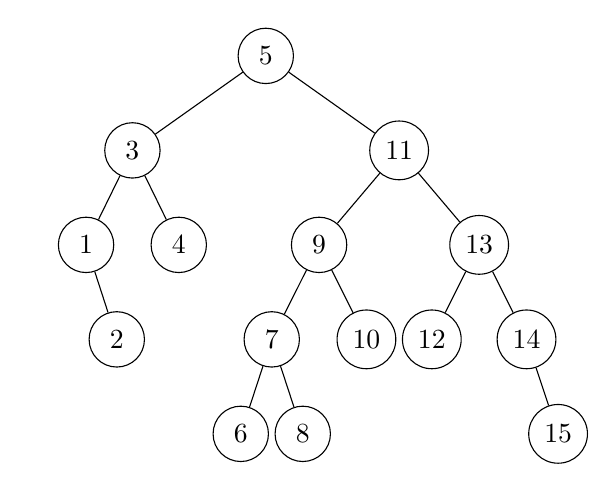
\begin{tikzpicture}[]
    \Tree
    [.5
        [.3
            [.1
                \edge[blank]; \node[blank]{};
                [.2
                ]
            ]
            [.4
            ]
        ]
        [.11
            [.9
                [.7
                    [.6
                    ]
                    [.8
                    ]
                ]
                [.10
                ]
            ]
            [.13
                [.12
                ]
                [.14
                    \edge[blank]; \node[blank]{};
                    [.15
                    ]
                ]
            ]
        ]
    ]
    \end{tikzpicture}
\end{center}

\begin{parts}

\part[2] Insert $8.5$ into $T$. Draw the AVL tree before checking if any balance correction is needed.

\begin{solution}

\vspace{2in}

\end{solution}

\part[2] Insert $8.5$ into $T$. Draw the AVL tree after balance corrections.
\begin{solution}

\vspace{2in}

\end{solution}

\part[2] Remove $3$ from $T$ (\textbf{NOT from the previous answer!}). Draw the AVL tree after replacing and before checking if any balance correction is needed.
\begin{solution}

\vspace{2in}


\end{solution}

\part[2] Remove $3$ from $T$. Draw the AVL tree after balance corrections.
\begin{solution}

\vspace{2in}

\end{solution}

\end{parts}

\titledquestion{Alphabet Cognitive Battle}

Consider the AVL tree below. Each symbol represents a unique object stored in the AVL tree.


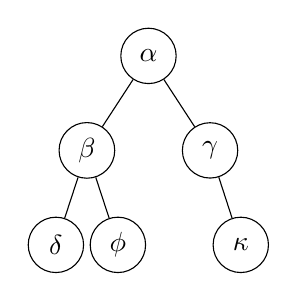
\begin{tikzpicture}[]
\Tree
[.$\alpha$
    [.$\beta$
        [.$\delta$
        ]
        [.$\phi$
        ]
    ]
    [.$\gamma$
        \edge[blank]; \node[blank]{};
        [.$\kappa$
        ]
    ]
]
\end{tikzpicture}

The following 4 questions are \textbf{independent} of each other, i.e. for each question, your answer should be built on the original AVL Tree above, instead of the AVL Tree from the answer of the last question.

\begin{parts}

\part[3] If we delete object $\gamma$, then insert object $\gamma$, then insert new object $\epsilon$ ($\gamma < \epsilon < \kappa$), please draw the AVL tree after each insert/delete operation.

\begin{solution}

\vspace{2in}

\end{solution}


\part[3] If we want to insert a new object $\epsilon$ (not equal to the 6 objects)but we don’t want to change the tree’s current structure to maintain balance. What are the ranges of the object we can insert? (Note: the range is denoted by the objects, for example, $\alpha < \epsilon < \beta, \epsilon < \delta)$.

\begin{solution}

\vspace{2in}

\end{solution}

\part[2] If we know the last object we insert is $\phi$. What is the tree before inserting it? Symbols must be unique. You may only use the 6 printed symbols. If there are more than 3 correct answers, giving only 3 correct answers would lead to full credit.

\begin{solution}

\vspace{2in}

\end{solution}


\part[3] If we don’t know the last object we insert, but we know we change the tree’s structure to maintain balance. What is the object we may insert? Please write down the possible objects. Symbols must be unique. You may only use the 6 printed symbols. If there are more than 3 correct answers, giving only 3 correct answers would lead to full credit. Giving any wrong answer will lead to zero credit.

\begin{solution}

\vspace{2in}

\end{solution}

\end{parts}

\end{questions}

\end{document}